\documentclass{article}

\usepackage{graphicx}
\usepackage{float}
\usepackage{amsmath}

%The following package imports and styling was obtained from: https://tex.stackexchange.com/questions/348651/c-code-to-add-in-the-document
\usepackage{xcolor}
\usepackage{listings}

\definecolor{mGreen}{rgb}{0,0.6,0}
\definecolor{mGray}{rgb}{0.5,0.5,0.5}
\definecolor{mPurple}{rgb}{0.58,0,0.82}
\definecolor{backgroundColour}{rgb}{0.95,0.95,0.92}

\usepackage[colorlinks]{hyperref}
\hypersetup{citecolor=DeepPink4}
\hypersetup{linkcolor=DarkRed}
\hypersetup{urlcolor=blue}
\usepackage{cleveref}

\lstdefinestyle{CStyle}{
    backgroundcolor=\color{backgroundColour},   
    commentstyle=\color{mGreen},
    keywordstyle=\color{magenta},
    numberstyle=\tiny\color{mGray},
    stringstyle=\color{mPurple},
    basicstyle=\footnotesize,
    breakatwhitespace=false,         
    breaklines=true,                 
    captionpos=b,                    
    keepspaces=true,                 
    numbers=left,                    
    numbersep=5pt,                  
    showspaces=false,                
    showstringspaces=false,
    showtabs=false,                  
    tabsize=2,
    language=C
}

\begin{document}
\title{Sfwr Eng 4F03: Final Project}

\author{Kelvin Lin\hspace{10mm}MacID:linkk4\hspace{10mm}Student Number: *********\\Prabhbir Pooni\hspace{10mm}MacID: poonip\hspace{10mm}Student Number: *********\\Yanting Zhang\hspace{10mm}MacID: zhang169\hspace{10mm}Student Number: *********}

\maketitle

\section{Question 1}
Using \texttt{MPIHost}, timing, speed-up, and efficiency plots were generated for 1, 2, 4, 8, 16, and 32 processors. The program was tested with 2000, 4000, 8000, 16000, and 32000 particles. 9 major steps were used with 1 substep in between. The image produced was 2550 pixels in width by 1960 pixels in height.

\subsection{Timing Plots}
The following graph is a timing plot for the different number of particles versus the different number of processors. Each line represents a different number of particles. The x-axis represents the number of processors while the y-axis represents the time it took to run the program.

\begin{figure}[H]
	\begin{center}
		\hspace*{-0.5cm}                                                           
  		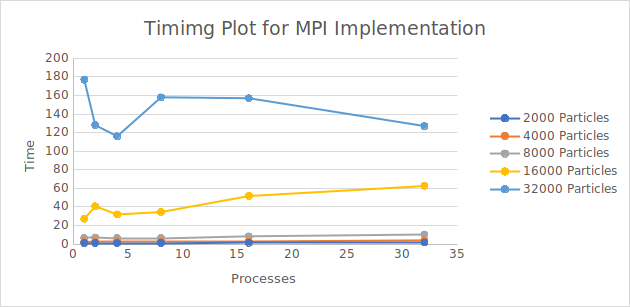
\includegraphics[scale=0.83]{Report_Assets/timingmpi.png}
  	\end{center}
  	\caption{The timing plot with varying the number of processors and particles}
\end{figure}


\end{document}
